\documentclass{beamer}
\usetheme{Madrid}
\usecolortheme{default}
\usepackage[utf8]{inputenc}
\usepackage{tikz}
\usepackage{circuitikz}
\usepackage{enumitem}
\usepackage{array}
\usepackage{amsmath}
\usepackage[export]{adjustbox}
\usetikzlibrary{arrows,shapes,automata,petri,positioning,calc}
\usetikzlibrary{positioning,shapes.gates.logic.US}

\colorlet{beamer@blendedblue}{blue!60!black}
\usebackgroundtemplate{
\includegraphics[width=\paperwidth,height=\paperheight]{img/assn11_bg.png}}

\tikzset{
    place/.style={
        circle,
        thick,
        draw=black,
        fill=gray!50,
        minimum size=6mm,
    },
        state/.style={
        circle,
        thick,
        draw=blue!75,
        fill=blue!20,
        minimum size=6mm,
    },
}

\title{assignment 11}
\subtitle{solution to gate EC 2014-2,question 9}
\author{dilip}
\date{January 2021}
\institute{IIIT RAICHUR}
\logo{
\includegraphics[height=1cm]{img/logo-blue-desktop.png}}

\AtBeginSection[]
{
  \begin{frame}
    \frametitle{Table of Contents}
    \tableofcontents[currentsection]
  \end{frame}
}
\begin{document}

\begin{frame}
\maketitle
\end{frame}

\section{Question}
\begin{frame}{Question Figure}
  \begin{figure}[h]
    \centering
    \scalebox{0.65}{
    \begin{tikzpicture}[
        GateCfg/.style={
            logic gate inputs={normal,normal,normal},
            draw,
            scale=1.5
        }
    ]
    
    % D flip flop 1
    \draw (0,0)coordinate (A)--++(0:3.5)coordinate (B)--++(90:4.5)coordinate (C)--++(180:3.5)coordinate (D)--cycle;
    \draw ($(A)!0.8!(D)$)node[right]{\Large D}--++(180:1.5)node[]{};
    \draw ($(A)!0.5!(C)$)node[]{\Large D Latch};
    \draw ($(B)!0.8!(C)$)node[left]{\Large Q}--++(0:4)node[]{};
    \draw ($(B)!0.2!(C)$)node[left]{\Large $\overline{\mbox{Q}}$}--++(0:0.5)node[]{};
    \draw ($(A)!0.53!(D)$)node[]{}--++(-30:0.3)node[]{}--++(-150:0.3)node[]{};
    \draw ($(A)!0.5!(D)$)node[]{}--++(180:1.5)node[]{};
    
    % D flip flop 2
    \draw (7.5,0)coordinate (A)--++(0:3.5)coordinate (B)--++(90:4.5)coordinate (C)--++(180:3.5)coordinate (D)--cycle;
    \draw ($(A)!0.8!(D)$)node[right]{\Large Q};
    \draw ($(A)!0.5!(C)$)node[]{\Large Q Latch};
    \draw ($(B)!0.8!(C)$)node[left]{\Large Q}--++(0:1.5)node[]{};
    \draw ($(B)!0.2!(C)$)node[left]{\Large $\overline{\mbox{Q}}$}--++(0:1.5)node[]{};
    \draw ($(A)!0.53!(D)$)node[]{}--++(-30:0.3)node[]{}--++(-150:0.3)node[]{};
    \draw ($(A)!0.5!(D)$)node[]{}--++(180:1.5)node[]{};
    
    % CLK
    \draw (-2.5,-1)node[below]{\Large CLK}node[]{}--++(0:1)node[]{}--++(90:3.25)node[]{};
    
    \draw (2,-1)node[not gate US,GateCfg](NOT){};
    \draw (-1.5,-1)node[]{}--(NOT.input)node[]{};
    \draw (NOT.output)node[]{}--++(0:3.35)node[]{}--++(90:3.27)node[]{};
    
\end{tikzpicture} }
    \caption{Question Diagram}
    \label{fig:my_label}
\end{figure}
\end{frame}

\begin{frame}{Question Text}
Current option is
\begin{enumerate}[label=(\alph*)]
    \item JK flip-flop
    \item SR flip-flop
    \item D flip-flop
    \item Master-slave arrangement
\end{enumerate}
\end{frame}

\section{Answer}
\begin{frame}{Answer} 
 The correct option is d)Master-slave arrangement.
 \end{frame}
 \subsection{Master-Slave D flip flop}
 \begin{frame}
 The basic D-type flip flop can be improved further by adding a second SR flip flop to its output that is activated on the complementary clock signal to produce a "Master-Slave D-type flip flop".On the leading edge of the clock signal( LOW-to-HIGH)the first stage, the "master" latches the input condition at D,while the output stage is deactivated.
  \par
 On the trailing edge of the clock signal (HIGH-to-LOW), the second "slave" stage is now activated, latching on to the output from the first master circuit.Then the output stage appears to be triggered on the negative edge of the clock pulse."Master-Slave D-type flip flop" can be constructed by the cascading together of two latches with opposite clock phases as shown.
\end{frame}
\subsection{Transition Table}
\begin{frame}{Transition Table}
    
\begin{table}[h]
\centering
\begin{tabular}{|lc|lc|}
\hline
Present State & Input & Next state & \multicolumn{1}{l|}{Output} \\
A   \;   B     & X     & A   \;  B    & Y                           \\ \hline
0   \:\:   0    & 0     & 0   \:\:  0    & 0                           \\
0   \:\:    0    & 1     & 0   \:\:  1    & 0                           \\
0    \:\:    1    & 0     & 0  \:\:   0    & 1                           \\
0    \:\:    1    & 1     & 1  \:\:  1    & 0                           \\
1    \:\:    0    & 0     & 0  \:\:   0    & 1                           \\
1    \:\:   0     & 1     & 1   \:\:  0    & 0                           \\
1     \:\:   1    & 0     & 0  \:\:  0     & 1                           \\
1     \:\:   1    & 1     & 1  \:\:  0     & 0                           \\ \hline
\end{tabular}

\label{tab:my-table}
\end{table}
\end{frame}

\subsection{State Diagram}
\begin{frame}{State Diagram}
 \begin{figure}[h]
    \centering
    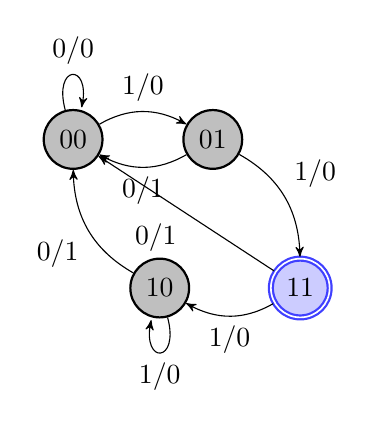
\begin{tikzpicture}[node distance=2cm and 1cm,>=stealth',auto, every place/.style={draw}]
    \node [place] (00) {00};
    \coordinate[node distance=1.1cm,left of=00](left-00);
    \coordinate[node distance=1.1cm,right of=00](right-00);
    
    \node [place] (01) [right=of 00] {01};
    \node [place] (10) [node distance=1.5cm,below =of right-00] {10};    
    \node [state,initial text=,accepting by double] (11) [right=of 10] {11};

    \path[->] (00) edge [bend left] node {1/0} (01);
    \path[->] (01) edge [bend left] node {0/1} (00);
    \path[->] (00) edge [loop above]node{0/0}();
    \path[->] (10) edge [bend left] node {0/1} (00);
    \path[->] (01) edge [bend left] node {1/0} (11);
    \path[->] (10) edge [loop below] node {1/0} ();
    \path[->] (11) edge [bend left] node {1/0} (10); 
    \path[->] (11) edge [] node{0/1}(00);
\end{tikzpicture}

    \caption{State Diagram}
    \label{fig:statediag}
 \end{figure}
\end{frame}

\begin{frame}{Timing Diagrams}
  \begin{figure}
    \centering
    \scalebox{0.3}{
        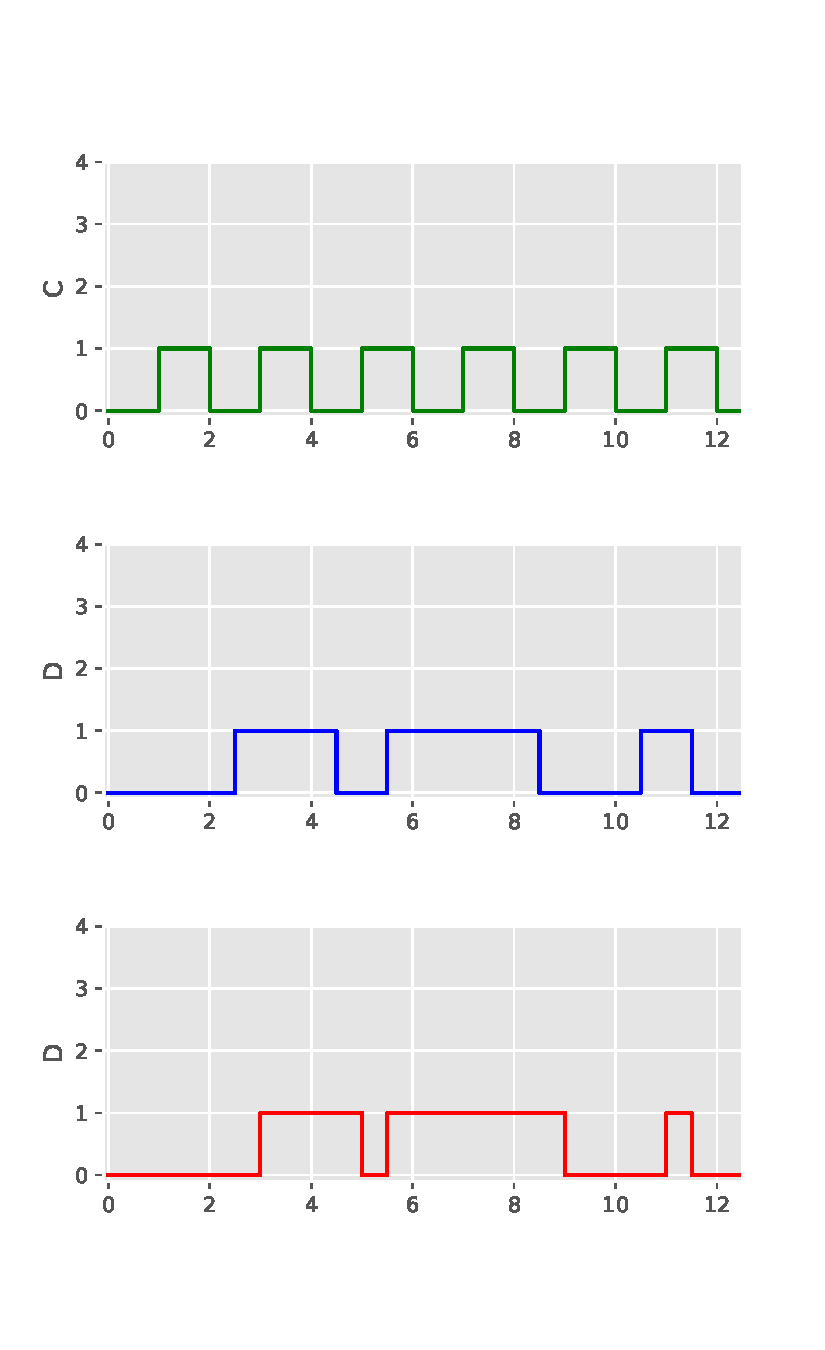
\includegraphics{figures/graph.pdf}}
   
    \caption{Timing diagram}
    \label{fig:my_label}
\end{figure}  
\end{frame}

\end{document}
